To begin identifying an appropriate development methodology, it is necessary to understand the project requirements. The project requirements are determined over a number of meetings with the primary stakeholders. These meetings discuss the minimum requirements and the features that are going to be implemented on the project. A more detailed reference on all the requirements is discussed in the previous section.

The next step is deciding the methodology that will be used. Since we are looking for iterative and incremental development, Agile Software Development Methodology will be followed. This also enables time-boxed iterative approach. Agile methods are focused on different aspects of the software development life cycle. Two of the most well known agile methodologies are Scrum and XP.

Scrum is a project management agile framework that focuses more on the management of software development projects. The product is completed in a series of one to four week iterations, or sprints. Before each sprint, a planning meeting is held to define which features will be implemented during that sprint. Similarly, XP (Extreme Programming) is an agile methodology which is designed for small, co-located teams aiming to get quality and productivity as high as possible. It does this through the use of rich, short, informal communication paths with emphasis on skill, discipline, and understanding at the personal level, minimizing all intermediate work products.

As this is a college project and tight time constraints apply, it is quite difficult to follow a particular methodology. Scrum focuses on the management side of the project whereas XP focuses more on the actual programming practices. It is more preferable if various elements from both methodologies will be used since they address different areas and complement each other.

Therefore, It was decided to focus on managing the software project using the scrum approach and adopt it's characteristics that suit the project. The team is composed by six students each one assigned with various tasks every week. Weekly meetings are also planned in order to organise the division of work and for the team to get up to speed with what every one is doing or completed. An agenda is stored in a document that holds the content and matters which the team discusses in each meeting.

To make the production more effective and faster, an online collaboration tool called "Trello" is used. This tool gives access to a visual board and displays all the required short-term or long-term tasks which are represented as cards with various labels and priorities. This board is very similar to the scrum board as shown in the following pictures:	

\begin{figure}[here]
\begin{minipage}{\textwidth}
\begin{center}
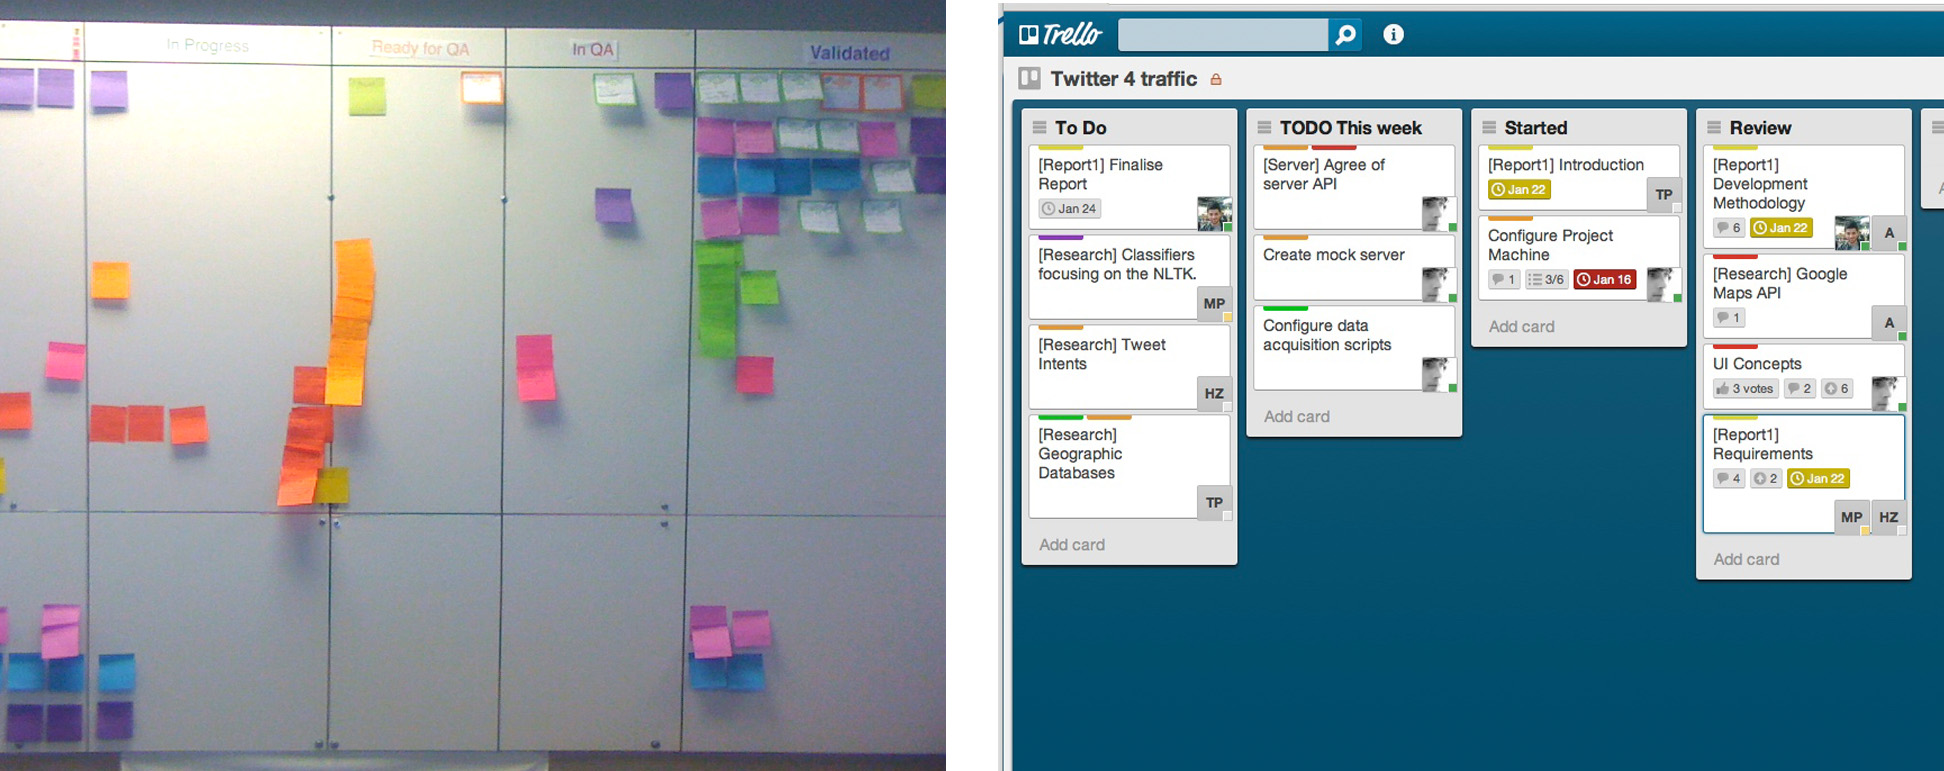
\includegraphics[width=0.8\textwidth]{images/scrumboard.jpg}
\end{center}
\vspace{-20pt}
\caption[Caption for LOF]{Scrum Board and Trello\footnotemark}
\end{minipage} 
\end{figure}


It has been also decided to adopt several techniques from the XP, which will help the improvement of the programming process. The first practise which has been decided to use is pair programming, having two programmers work alongside on the same code. At any time, those two programmers sitting together may change any line of code in the system. Any time the two find a section of code that appears hard to understand or overly complex, they are to revise it, constantly simplifying and improving it. Furthermore, several tests will be added in the code-base, keeping a test-driven development . However because of the nature of the project being partly research based and the results being quite subjective, it is difficult to test effectively. Hence, the development of the mobile application will be a TDD whereas for the server will be followed a less strictly test-drive development.\cite{Cockburn}

For the division of work amongst the project, more flexibility will be achieved by maximising the use of the members previous experience, but also keeping everyone interested. A balanced division has been decided where two members of the team will focus on the mobile application, two on the server side and the rest will move between those two tasks as necessary.

To achieve parallel development, the server API will be mocked-up and will produce a fixed data set in the desired format that the android applications can handle. That way, those developing the mobile application can work independently from those working on the server. One person on the team is designated as the team "coach". This person reviews with the team members their use of the key practices: use of pair programming and testing,keeping design simple, communicating, and so on.

As regards the mobile application that will act as the front-end of the system, some Lo-Fi layouts will be drawn in paper in order to have a general idea of how the interface is going to look like. The relative data will be retrieved in a structured format that will be the identical for the server and the mobile application.

\footnotetext{Left: Drew Stephens \url{flickr.com/photos/dinomite/3695570625}, Right: \copyright \url{Trello.com}}
